\begin{figure}[t]
  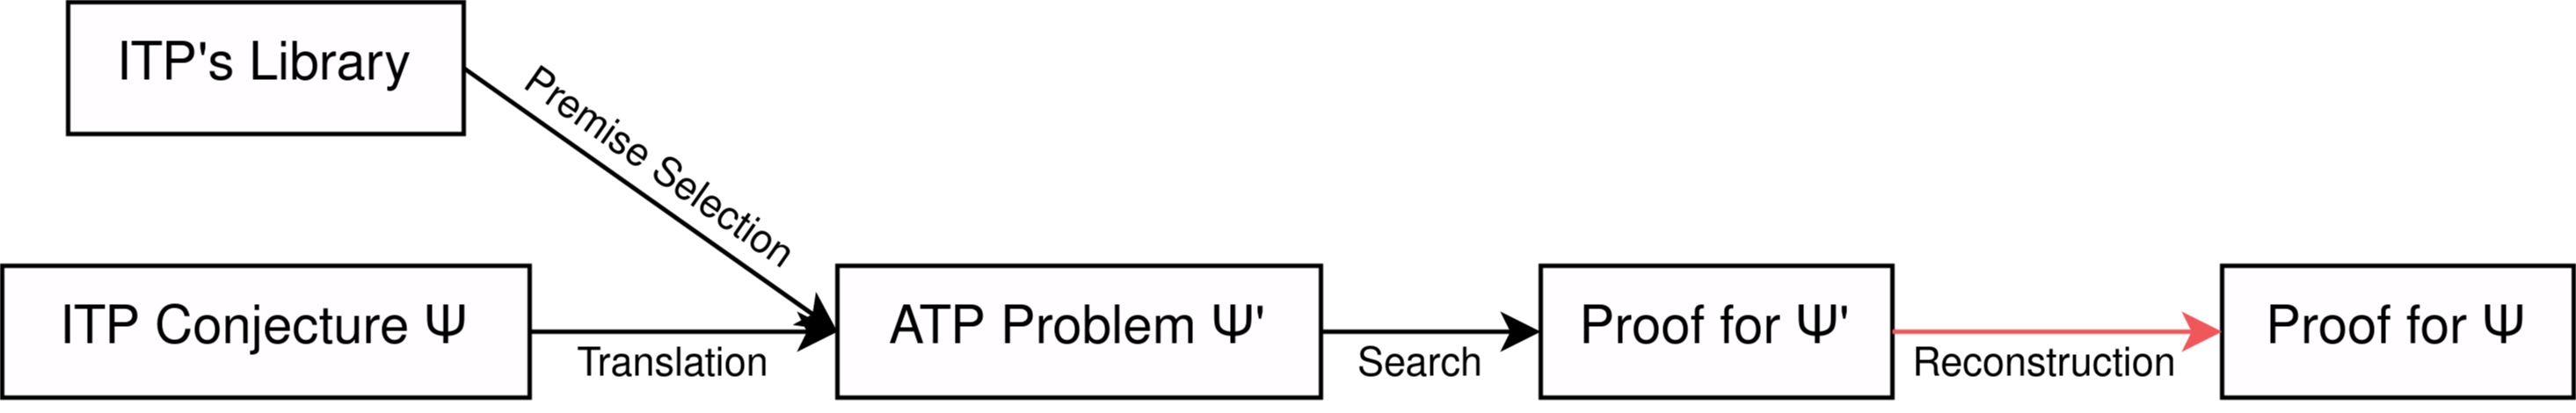
\includegraphics[scale=0.15]{img/hammerArch.png}
  \caption{General Architecture of a Hammer}\label{fig:archHamm}
\end{figure}

\label{sec:hammering}

% The paper Hammering Towards QED~\cite{hammering} describes
% the most relevant ones and also outlines
% all the efforts that were already made in order to integrate
% interactive and automatic theorem provers. The authors employ
% this information to provide a detailed description of each
% component that must be implemented in a system establishing
% a connection between ATPs and ITPs. Furthermore, this work
% presents a series of benchmarks showing the potential of these
% tools. These benchmarks tipically involve selecting a set
% of theorems proved in the ITP's library and checking how often the
% tool can find a proof for them without human interaction.
% Some experiments demonstrated that there are theorems for which
% the ATP can even find a proof shorter than those found in the ITP's library.

Systems whose purpose is to discharge the responsibility of proving theorems stated in
an interactive theorem prover to an automatic one are known as ``hammers''~\cite{hammering}.
Given a conjecture $\psi$ to be proven inside an ITP, a hammer will execute the following three steps:

\begin{itemize}
  \item First, it will inspect the library of theorems already proven inside the ITP
        and heuristically select the ones that are more relevant to prove $\psi$.
        Usually, the ATP will not be aware of the existence of these theorems, so it is
        possible to facilitate the process of searching for a proof by adding them as
        hypothesis to the problem. The module responsible for this process is known as the
        \textbf{premise selection module}.\@
  \item Once the premisses are selected, the hammer will translate $\psi$ into a problem
        $\psi'$ expressed in a language recognized by the ATP. The problem $\psi'$ must
        be equivalent to $\psi$, with all the premisses that were selected in the previous step
        added as hypothesis. This is done by the \textbf{translation module}.\@
  \item Next, $\psi'$ will be fed to the automatic theorem prover. The solver will then try to
        verify the correctness of the conjecture or find a counterexample, producing a
        certificate supporting the result it found.
        If the ATP could validate the conjecture, then the
        certificate will be a proof. In this case, the hammer will use the
        \textbf{proof reconstruction module} to reconstruct this proof inside
        the interactive theorem prover as a proof for $\psi$.

\end{itemize}

This workflow is summarized in Figure~\ref{fig:archHamm}.

In this dissertation we describe how we implemented a proof reconstruction module
for Lean users from cvc5 proofs.
The two main strategies used to reconstruct the proof produced
by the automatic system inside the interactive are also well-known:
The first one is known as the \textit{certified} approach~\cite{snipe}. In this case,
the hammer defines a datatype to represent
terms in the language of the ATP and a set of functions to manipulate
values of those datatypes, representing
the inference rules that the solver uses to reason about those terms. Then, a lifting function is defined, that is,
a function that takes a value of this datatype and outputs an equivalent term in the native
language of the ITP.\ Finally, the correctness of each function is
verified with respect to the lifting function, in the sense that, if the input term
was lifted to a value that is true in the ITP's logic, then the output term will
also be true. The ATP's proof will be represented as a sequence of applications of those
functions, and their correctness are proved \textit{a priori}. When checking
a specific proof, the only step that the hammer must perform is to compute the result
of the application of all the functions in the solver's output, and to check if
the final term matches with the expected one.

The second approach is known as the \textit{certifying} approach~\cite{snipe}. It consists of matching
each axiom in the ATP's logic into tactics
defined in the ITP that operate directly over native terms of the system and parsing
the proof produced by the automatic solver into a sequence of applications
of those tactics, which are replayed inside the ITP.\
Those tactics rely on theorems previously proved inside the ITP to simulate the ATP's inference rules.
In this case, the proof steps are reconstructed and checked in the ITP on the
fly each time the hammer is invoked. Since there is no theorem stating the
correctness of them, it is possible that this process fails.
On the other hand,
this technique skips computations over embedded terms which have to be done by the
certified approach, granting it the potential to have a better
performance~\cite{ringLean}. It also diminishes the complexity of the tool, as there is no need to
define an intermediate representation inside the ITP.\

We present implementations of the certified and certifying approaches in Lean
in Chapters~\ref{chap:certified} and~\ref{chap:rcons}, respectively. For reasons
we will explain in the later chapters, our main focus is on the certifying approach.

The next two sections describe examples of hammers.
Both of these works exhibit similarities to our research, therefore, it is useful to reference them here.
It is important to note that both of these are established hammers, and teams have been working on optimizing their
performance for years. As we have previously pointed out, the primary objective of our system is to cover the largest
range of proofs produced by cvc5 as opposed to having the best possible performance.
Therefore, due to the time constraints of this project, improving the
efficiency of our module is left for future work, so the current system is slower than
the other hammers.
%
In Section~\ref{chap:future}, we discuss ideas to improve this aspect of our tool.
